% ŠABLONA PRO PSANÍ ZÁVĚREČNÉ STUDIJNÍ PRÁCE
%%%%%%%%%%%%%%%%%%%%%%%%%%%%%%%%%%%%%%%%%%%%
% Autor: Jakub Dohulil (kubadokulil99@gmail.com)
% Tato šablona byla vytvořena tak, aby pomocí ní mohli v systému LaTeX soutěžící sázet své práce a zároveň odpovídala požadavkům na formátování vyplývajícím z wordové šablony umístěné na webu soc.cz.
%
\documentclass[12pt, a4paper,
%oneside,      %% -- odkomentujte, pokud chcete svou práci mít pouze jednostrannou, mezera pro hřbet pak automaticky bude pouze na levé straně
twoside        %% -- pro oboustranné práce, mezera pro hřbet následně střídá strany.
]{report}

%% Nutné balíčky a nastavení
%%%%%%%%%%%%%%%%%%%%%%%%%%%%

%% Proměnné
\newcommand\obor{INFORMAČNÍ TECHNOLOGIE} %% -- napiš číslo a název tvého oboru
\newcommand\kodOboru{18-20-M/01} %% -- napiš číslo a název tvého oboru
\newcommand\zamereni{se zaměřením na počítačové sítě a programování} %% -- napiš číslo a název tvého oboru
\newcommand\skola{Střední škola průmyslová a umělecká, Opava} %% vyplň název školy
\newcommand\trida{IT4} %% vyplň jméno svého konzultanta
\newcommand\jmenoAutora{Aleš Najser}  %% vyplň své jméno
\newcommand\skolniRok{2023/24} %% vyplň rok
\newcommand\datumOdevzdani{1. 1. 2024} %% vyplň rok
\newcommand\nazevPrace{MazeRoller} %% vyplň název své práce

\title{\nazevPrace} %% -- Název tvé práce
\author{\jmenoAutora} %% -- tvé jméno
\date{\datumOdevzdani} %% -- rok, kdy píšeš SOČku

% Předefinování příkazu chapter
\let\oldchapter\chapter
\renewcommand{\chapter}{
\clearpage
\pagestyle{plain}
\oldchapter
}


\usepackage[top=2.5cm, bottom=2.5cm, left=3cm, right=3cm]{geometry} %% nastaví okraje, left -- vnitřní okraj, right -- vnější okraj

\usepackage[czech]{babel} %% balík babel pro sazbu v češtině
\usepackage[utf8]{inputenc} %% balíky pro kódování textu
\usepackage[T1]{fontenc}
\usepackage{cmap} %% balíček zajišťující, že vytvořené PDF bude prohledávatelné a kopírovatelné

\usepackage{graphicx} %% balík pro vkládání obrázků

\usepackage{subcaption} %% balíček pro vkládání podobrázků

\usepackage{hyperref} %% balíček, který v PDF vytváří odkazy

\linespread{1.25} %% řádkování
\setlength{\parskip}{0.5em} %% odsazení mezi odstavci



\usepackage[pagestyles]{titlesec} %% balíček pro úpravu stylu kapitol a sekcí
\titleformat{\chapter}[block]{\scshape\bfseries\LARGE}{\thechapter}{10pt}{\vspace{0pt}}[\vspace{-22pt}]
\titleformat{\section}[block]{\scshape\bfseries\Large}{\thesection}{10pt}{\vspace{0pt}}
\titleformat{\subsection}[block]{\bfseries\large}{\thesubsection}{10pt}{\vspace{0pt}}


\usepackage{tocloft} % Balíček umožní přizpůsobit vzhled tabulky obsahu
\setlength{\cftbeforechapskip}{0pt}  % Menší rozestup pro kapitoly
\setlength{\cftbeforesecskip}{0pt}   % Menší rozestup pro sekce

\setcounter{secnumdepth}{2}
\setcounter{tocdepth}{2}
\usepackage{fancyhdr}
\pagestyle{fancy}
\renewcommand{\headrulewidth}{0.025pt}

\usepackage{booktabs}

\usepackage{url}

%% Balíčky co se můžou hodit :) 
%%%%%%%%%%%%%%%%%%%%%%%%%%%%%%%

\usepackage{pdfpages} %% Balíček umožňující vkládat stránky z PDF souborů, 

\usepackage{upgreek} %% Balíček pro sazbu stojatých řeckých písmen, třeba u jednotky mikrometr. Například stojaté mí: \upmu, stojaté pí: \uppi

\usepackage{amsmath}    %% Balíčky amsmath a amsfonts 
\usepackage{amsfonts}   %% pro sazbu matematických symbolů
\usepackage{esint}     %% pro sazbu různých integrálů (např \oiint)
\usepackage{mathrsfs}
\usepackage{helvet} % Helvet font
\usepackage{mathptmx} % Times New Roman
\usepackage{Oswald} % Oswald font


%% makra pro sazbu matematiky
\newcommand{\dif}{\mathrm{d}} %% makro pro sazbu diferenciálu, místo toho
%% abych musel psát '\mathrm{d}' mi stačí napsat '\dif' což je mnohem 
%% kratší a mohu si tak usnadnit práci

\usepackage{listings}
\usepackage{xcolor}

\renewcommand{\lstlistingname}{Kód}% Listing -> Algorithm
\renewcommand{\lstlistlistingname}{Seznam programových kódů}% List of Listings -> List of Algorithms

%% Definice 
\lstdefinelanguage{JavaScript}{
	morekeywords=[1]{break, continue, delete, else, for, function, if, in,
		new, return, this, typeof, var, void, while, with},
	% Literals, primitive types, and reference types.
	morekeywords=[2]{false, null, true, boolean, number, undefined,
		Array, Boolean, Date, Math, Number, String, Object},
	% Built-ins.
	morekeywords=[3]{eval, parseInt, parseFloat, escape, unescape},
	sensitive,
	morecomment=[s]{/*}{*/},
	morecomment=[l]//,
	morecomment=[s]{/**}{*/}, % JavaDoc style comments
	morestring=[b]',
	morestring=[b]"
}[keywords, comments, strings]


\lstdefinelanguage[ECMAScript2015]{JavaScript}[]{JavaScript}{
	morekeywords=[1]{await, async, case, catch, class, const, default, do,
		enum, export, extends, finally, from, implements, import, instanceof,
		let, static, super, switch, throw, try},
	morestring=[b]` % Interpolation strings.
}

\lstalias[]{ES6}[ECMAScript2015]{JavaScript}

% Nastavení barev
% Requires package: color.
\definecolor{mediumgray}{rgb}{0.3, 0.4, 0.4}
\definecolor{mediumblue}{rgb}{0.0, 0.0, 0.8}
\definecolor{forestgreen}{rgb}{0.13, 0.55, 0.13}
\definecolor{darkviolet}{rgb}{0.58, 0.0, 0.83}
\definecolor{royalblue}{rgb}{0.25, 0.41, 0.88}
\definecolor{crimson}{rgb}{0.86, 0.8, 0.24}


% Nastavení pro c sharp

\usepackage{listings}
\usepackage{color}
\lstloadlanguages{C,C++,csh,Java}

\definecolor{red}{rgb}{0.6,0,0} 
\definecolor{blue}{rgb}{0,0,0.6}
\definecolor{green}{rgb}{0,0.8,0}
\definecolor{cyan}{rgb}{0.0,0.6,0.6}

\lstset{
language=csh,
basicstyle=\footnotesize\ttfamily,
numbers=left,
numberstyle=\tiny,
numbersep=5pt,
tabsize=2,
extendedchars=true,
breaklines=true,
frame=b,
stringstyle=\color{blue}\ttfamily,
showspaces=false,
showtabs=false,
xleftmargin=17pt,
framexleftmargin=17pt,
framexrightmargin=5pt,
framexbottommargin=4pt,
commentstyle=\color{green},
morecomment=[l]{//}, %use comment-line-style!
morecomment=[s]{/*}{*/}, %for multiline comments
showstringspaces=false,
morekeywords={ abstract, event, new, struct,
as, explicit, null, switch,
base, extern, object, this,
bool, false, operator, throw,
break, finally, out, true,
byte, fixed, override, try,
case, float, params, typeof,
catch, for, private, uint,
char, foreach, protected, ulong,
checked, goto, public, unchecked,
class, if, readonly, unsafe,
const, implicit, ref, ushort,
continue, in, return, using,
decimal, int, sbyte, virtual,
default, interface, sealed, volatile,
delegate, internal, short, void,
do, is, sizeof, while,
double, lock, stackalloc,
else, long, static,
enum, namespace, string},
keywordstyle=\color{cyan},
identifierstyle=\color{red},
backgroundcolor=\color{white},
}

\usepackage{caption}
\DeclareCaptionFont{white}{\color{white}}
\DeclareCaptionFormat{listing}{\colorbox{blue}{\parbox{\textwidth}{\hspace{15pt}#1#2#3}}}
\captionsetup[lstlisting]{format=listing,labelfont=white,textfont=white, singlelinecheck=false, margin=0pt, font={bf,footnotesize}}


\lstdefinestyle{JSES6Base}{
	backgroundcolor=\color{white},
	basicstyle=\ttfamily,
	breakatwhitespace=false,
	breaklines=false,
	captionpos=b,
	columns=fullflexible,
	commentstyle=\color{mediumgray}\upshape,
	emph={},
	emphstyle=\color{crimson},
	extendedchars=true,  % requires inputenc
	fontadjust=true,
	frame=single,
	identifierstyle=\color{black},
	keepspaces=true,
	keywordstyle=\color{mediumblue},
	keywordstyle={[2]\color{darkviolet}},
	keywordstyle={[3]\color{royalblue}},
 literate=%
{á}{{\'a}}1 {č}{{\v{c}}}1 {ď}{{\v{d}}}1 {é}{{\'e}}1 {ě}{{\v{e}}}1
{í}{{\'i}}1 {ň}{{\v{n}}}1 {ó}{{\'o}}1 {ř}{{\v{r}}}1 {š}{{\v{s}}}1
{ť}{{\v{t}}}1 {ú}{{\'u}}1 {ů}{{\r{u}}}1 {ý}{{\'y}}1 {ž}{{\v{z}}}1,		
	numbers=left,
	numbersep=5pt,
	numberstyle=\tiny\color{black},
	rulecolor=\color{black},
	showlines=true,
	showspaces=false,
	showstringspaces=false,
	showtabs=false,
	stringstyle=\color{forestgreen},
	tabsize=2,
	title=\lstname,
	upquote=true  % requires textcomp
}

\lstdefinestyle{JavaScript}{
	language=JavaScript,
	style=JSES6Base,
}
\lstdefinestyle{ES6}{
	language=ES6,
	style=JSES6Base
}


%% Bordel pro práci - můžeš smáznout :) 
%%%%%%%%%%%%%%%%%%%

\usepackage{lipsum} %% balíček který píše lipsum (nesmyslný text, který se používá pro kontrolu typografie)

%% Začátek dokumentu
%%%%%%%%%%%%%%%%%%%%
\begin{document}
	
	\pagestyle{empty}
	\pagenumbering{Roman}
	
	\cleardoublepage

%% Titulní stránka s informacemi
%%%%%%%%%%%%%%%%%%%%%%%%%%%%%%%%%%%%%%%%
	
	{\fontfamily{phv}\selectfont
		%% Logo školy
		\begin{figure}[h]
			\centering
			
\includegraphics[width=0.6\linewidth]{image/logo-skoly.png} 
		\end{figure}
		
		
		%% Hlavička práce a její název (viz proměnná \nazev prace)
		%% \sffamily %%% bezpatkové písmo - sans serif
		{\bfseries %%% písmo na stránce je tučně
			\begin{center}
				\vspace{0.025 \textheight}
				\LARGE{ZÁVĚREČNÁ STUDIJNÍ PRÁCE}\\
				\large{dokumentace}\\
				\vspace{0.075 \textheight}
				\LARGE {\nazevPrace}\\
			\end{center}  
		}%%%
		
		\begin{figure}[h]
			\centering
			
\includegraphics[width=0.8\linewidth, height=3in]{image/mazeroller.jpg} 
		\end{figure}
		
		\vspace{0.02 \textheight}
		\begin{table}[h!]
			\begin{tabular}{ll}
				\textbf{Autor:} & \jmenoAutora\\ 
				\textbf{Obor:} & \kodOboru { } \obor\\
				\textbf{} & \zamereni\\
				\textbf{Třída:} & \trida\\
				\textbf{Školní rok:} & \skolniRok\\
			\end{tabular}
			
		\end{table}		
	}
	
\cleardoublepage %% Zalomení dvojstránky
	
%% Stránka obsahující poděkování a prohlášení
%%%%%%%%%%%%%%%%%%%%%%%%%%%%%%%%%%%%%%%%%%%%%%%%%%%%%%%%

%% Poděkování - nepovinné
%%%%%%%%%%%%%%%%%%%%%%%%%%%%
	
	\noindent{\large{\bfseries{Poděkování}\\}}
	\noindent Poděkovat bych chtěl hned několika lidem. Jmenovitě:
     \begin{itemize}
    	\item Marek Lučný - konzultace ohledně úvodní myšlenky a usměrnění cílů.
    	\item Marcel Godovský - konzultace ohledně hardwarových částí projektu.
    	\item David Kanovský - pomoc při studování C\#.
    	\item Jiří Ryba - pomoc s vytvořením obalu na hardwarové součástky.
    \end{itemize}
	
	\vspace*{0.5\textheight} %% Vertikální mezeru je možné upravit

%% Prohlášení - povinné
%%%%%%%%%%%%%%%%%%%%%%%%%%%%
	\noindent{\large{\bfseries{Prohlášení}\\}}  %% uprav si koncovky podle toho na jaký rod se cítíš, vypadá to pak lépe :) 
	\noindent{Prohlašuji, že jsem závěrečnou práci vypracoval samostatně a uvedl veškeré použité 
		informační zdroje.\\}
	\noindent{Souhlasím, aby tato studijní práce byla použita k výukovým a prezentačním účelům na Střední průmyslové a umělecké škole v Opavě, Praskova 399/8.}
	\vfill
	\noindent{V Opavě \datumOdevzdani\\}
	\noindent
	\begin{minipage}{\linewidth}
		\hspace{9.5cm} 
		\begin{tabular}{@{}p{6cm}@{}}
			\dotfill \\
			Podpis autora
		\end{tabular}
	\end{minipage}
	
	\cleardoublepage %% Zalomení dvojstránky

%% Stránka obsahující abstrakt (anotaci)
%%%%%%%%%%%%%%%%%%%%%%%%%%%%%%%%%%%%%%%%%%%%%%%%%%%%%%%%	

%% Abstrakt v češtině
%%%%%%%%%%%%%%%%%%%%%%%%%%%%
	\noindent{\Large{\bfseries{Abstrakt}\\}}
	Tento projekt v Unity využívá algoritmus pro generování labyrintu, ve kterém hráč ovládá kuličku pomocí hardwarového ovladače. Hráč se snaží dostat kuličku do cíle labyrintu. Samotný labyrint má možnost dvou velikostí a to 10x10 a 20x20.\\
	Se zvětšeným labyrintem se zvýší počet překážek a kamera se oddálí, aby bylo vidět celé hrací pole. Labyrint je taky opatřen generací cíle, který se může generovat pouze s určitou vzdáleností od hráče a určitého počtu překážek.\\
    K projektu je také hardwarový ovladač složen z arduina a akcelerometru. Hra automaticky detekuje port na kterém je ovladač připojen a poté odesílá informace o naklonění ovladače přímo do unity, kde se s pomocí těchto informací pohybuje kulička v labyrintu.\\
    
	
	\vspace{18pt}
	
	\noindent{\large{\bfseries{Klíčová slova}}}
	
	\noindent Unity, 3D, Hardware, Hra, Arduino, Labyrint, Depth-first algoritmus
	
	\pagebreak


%% Stránka s generovaným obsahem
%%%%%%%%%%%%%%%%%%%%%%%%%%%%%%%%%%%%%%%	
	
	\tableofcontents %% Vygeneruje tabulku s obsahem

	\pagenumbering{arabic} %% Nastavení způsobu číslování stránek (alternativy roman | Roman)
	\setcounter{page}{1} %% Nastavení počitadla stránek

%% Stránka s úvodem - povinná část
%%%%%%%%%%%%%%%%%%%%%%%%%%%%%%%%%%%%%%%		
	\chapter*{Úvod}
%Tento příkaz vytvoří novou kapitolu s názvem "Úvod" ve vašem dokumentu.
%Hvězdička * u příkazu \chapter* znamená, že tato kapitola nebude mít číslo. Ve výsledném dokumentu se tedy objeví jako "Úvod" bez předcházejícího čísla kapitoly, které se obvykle zobrazuje u číslovaných kapitol.
%Tento příkaz také znamená, že kapitola se automaticky neobjeví v obsahu, protože LaTeX standardně zahrnuje do obsahu pouze číslované kapitoly.
	\addcontentsline{toc}{chapter}{Úvod}
%Tento příkaz ručně přidává záznam do obsahu.
%První parametr toc označuje, že přidáváme záznam do Table of Contents (obsahu).
%Druhý parametr chapter specifikuje úroveň záznamu. V tomto případě říkáme, že přidávaný záznam má být považován za kapitolu.
%Třetí parametr Úvod je text, který se objeví v obsahu. V tomto případě bude v obsahu zobrazen název "Úvod".	
Unity je vynikající platforma pro vytváření 2D i 3D her, což získalo popularitu díky bezplatné licenci, kterou si může přisvojit kdokoli, dokud z jeho tvorby nevynese více než 100,000\$ ročně. Tento limit byl nedávno zvýšen na 200,000\$ za rok. \\
Jeho uživatelsky přívětivé prostředí umožňuje snadnou tvorbu her pomocí grafického rozhraní. V případě potřeby složitějších funkcí si však uživatel může vytvořit vlastní C\# skripty, což umožňuje kompletní kontrolu nad vývojem. \\
Mě osobně fascinuje vývoj her a zejména jejich funkčnost. Toužil jsem pochopit, jak lze propojit vytvořený ovladač s počítačem a využívat ho k ovládání prvků her. Tímto rozhodnutím jsem se rozhodl tuto problematiku prozkoumat na vlastní kůži a vytvořit vlastní hru, která by poskytla unikátní herní zážitek díky originálnímu ovladači. \\
Dokumentace je rozdělena do čtyř kapitol:
\begin{itemize}
\item První kapitola obsahuje srozumitelné vysvětlení algoritmu použitého pro vytvoření náhodného labyrintu a jeho praktické využití.
\item Druhá kapitola popisuje proces generace objektů v labyrintu.
\item Třetí kapitola se věnuje použitým součástkám a vysvětluje, proč a jak byly určité součástky využity.
\item Čtvrtá kapitola detailně popisuje propojení programu Unity se sériovým portem Arduina a jejich vzájemnou komunikaci.
\end{itemize}

%Tipy k psaní úvodu
%Je povinný, nadpis neměňte, rozsah - max. 1 strana. 
%Tato část práce obsahuje: 
%* náhled do řešené problematiky, zdůvodnění volby problematiky, 
%* předem definované cíle práce, 
%* motivaci pro další čtení textu včetně stručného uvedení obsahu následujících kapitol 


\chapter{Generování labyrintu}

\section{Recursive backtracker algoritmus}
\label{sec:recursive_backtracker_algoritmus}

{"Recursive backtracker" algoritmus.}Labyrint je generován díky takzvanému "recursive backtracker" algoritmu. Algoritmus funguje následovně : představme si že máme velkou mřížku (v případě mého projektu 10x10 nebo 20x20). V této mřížce si vybereme náhodnou polohu jedné škatulky.Z této škatulky dále vybereme další kostičku do které budeme postupovat. Nyní si tento pohyb na druhou kostku poznamenáme ať víme jak jsme se tam dostali a odebereme stěnu mezi těmito kostkami. A znovu se opakuje tento proces dokud nenarazíme na tzv. "slepou uličku", odkud se nemáme kam pohnout. V tomto případě se pomalu vracíme po naší cestě zpět dokud nenajdeme další kostku do které můžeme postoupit a označíme již prošlou cestu jako hotovou, jelikož již nemá žádné možné cesty. Tento proces se opakuje dokud algoritmus neprojde všechny možné cesty, tudíž se bude muset vrátit zpět na startovní políčko a ukončí se. 

\begin{figure}[h]
    \centering
    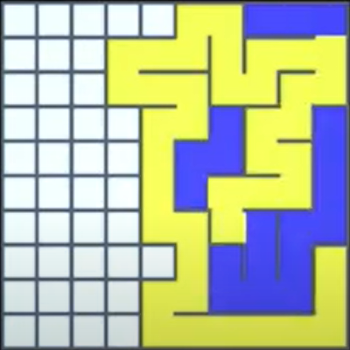
\includegraphics[height=0.3\textheight]{image/maze_generation.png}
    \caption\centering{Vizualizace algoritmu, kde žlutá znamená políčko s jedním navštívením, modré políčko znázorňuje hotovou cestu (2 návštěvy) a bílé políčka ještě nebyly navštíveny.}
\end{figure}

\vspace{0.1in}


\subsection{Vytvoření mřížky labyrintu}
Pro využití teorie již zmíněného algoritmu budeme muset sepsat třídu pro generování labyrintu. Nejdříve ale potřebujeme 
následovně vytvořit mřížku:
\begin{lstlisting}[language={[Sharp]C}, caption={C\# Vytvoření nodů (mřížky)}, label={Script}]
List<MazeNode> nodes = new List<MazeNode>();
        for (int x = 0; x < size.x; x++)
        {
            for (int y = 0; y < size.y; y++)
            {
                Vector3 nodePos = new Vector3(x - (size.x / 2f), 0, y - (size.y / 2f));
                MazeNode newNode = Instantiate(nodePrefab, nodePos, Quaternion.identity, transform);
                nodes.Add(newNode);

            }
        }
\end{lstlisting}

\subsection{Vyhledání možné cesty}
Jakmile je vytvořena mřížka můžeme začít hledat cestu. K tomuto je potřeba zjistit kterým směrem se můžeme a naopak nemůžeme pohnout. Takto lze například zjistit zda políčko napravo od naší momentální pozice vyhovuje našim podmínkám pro další pohyb:

\begin{lstlisting}[language={[Sharp]C}, caption={C\# příklad hledání cesty}, label={Script}]
if(currentNodeX < size.x - 1)
{
    if (!completedNodes.Contains(nodes[currentNodeIndex + size.y])&& !currentPath.Contains(nodes[currentNodeIndex + size.y]))
    {
        possibleDirections.Add(1);
        possibleNextNodes.Add(currentNodeIndex + size.y);
        }
}   
\end{lstlisting}

\vspace{1in}

\subsection{Odstranění stěny při pohybu skrz labyrint}
Při pohybu skrz labyrint je třeba odstranit stěnu pro vygenerování cesty. Toto je řešeno pomocí scriptu NodeState, který příjme status nodu (škatulky) a dále provede předdefinovanou akci.
\begin{lstlisting}[language{[Sharp]C}, caption={C\# Nastavení NodeState}, label={Script}]
    switch (state){
        case NodeState.Finish:
            floor.GetComponent<MeshRenderer>().material.color = Color.blue;
            floorWithHole.gameObject.SetActive(false);
            this.gameObject.tag = "Finish";
            break;
        case NodeState.Obstacle:
            floor.gameObject.SetActive(false);
            break;
        }
    }
\end{lstlisting}

\chapter{Generace objektů v labyrintu}
\section{Náhodné vytvoření cíle v labyrintu}
Každý labyrint by měl mít svůj konec v tomto projektu je náhodné generování labyrintu řešeno podobným způsobem jako generování překážek o kterém se znovu zmíním v další sekci. kód pro generaci cíle vypadá následovně:

\begin{lstlisting}[language={[Sharp]C}, caption={C\# Vytváření náhodných překážek v labyrintu}, label={Script}]
MazeNode randomCompletedNodeFinish = completedNodes[Random.Range(0, completedNodes.Count)];

        // Calculate the distance between the object's position and Vector3.ZERO
        float distanceToZero = Vector3.Distance(randomCompletedNodeFinish.transform.position, Vector3.zero);

        // Choose a random completed node to place the object as long as it's at least 3 units away from Vector3.ZERO
        while(distanceToZero < 3){
            randomCompletedNodeFinish = completedNodes[Random.Range(0, completedNodes.Count)];

            distanceToZero = Vector3.Distance(randomCompletedNodeFinish.transform.position, Vector3.zero);
        }   

        // Change the color of the chosen node for better visibility of the finish node
        randomCompletedNodeFinish.SetState(NodeState.Finish);
\end{lstlisting}

\vspace{1in}


\section{Náhodné vytvoření překážek v labyrintu}
Také je potřeba v labyrintu generovat náhodně překážky, aby nebyl příliš jednoduchý. Kód musí být opatřen aby se nevytvořila překážka na startu ani konci labyrintu.
\begin{lstlisting}[language={[Sharp]C}, caption={C\# Vytváření náhodných překážek v labyrintu}, label={Script}]
for(int i = 0; i<(size.x * size.y / 10); i++){
    MazeNode randomCompletedNode = completedNodes[Random.Range(0, completedNodes.Count)];
    if(randomCompletedNode.transform.position != randomCompletedNodeFinish.transform.position && randomCompletedNode.transform.position != Vector3.zero){
        randomCompletedNode.SetState(NodeState.Obstacle);
    }
}
\end{lstlisting}

\section{Death bariéra}
Jakmile máme v labyrintu překážky díky které může hráč vypadnout mimo labyrint, je potřeba přidat možnost restartovat hru od začátku. Přesně proto jsou potřeba death bariéry, které hráči oznámí že hru prohrál a pokud chce pokračovat musí začít od znovu.
Toto jsem vyřešil pomocí C\# skriptu který detekuje zda se hráč dotýka objektu který má tag "DeathBorder":
\begin{lstlisting}[language={[Sharp]C}, caption={C\# skript pro detekování hráče v death borderu}, label={Script}]
if (gameObject.CompareTag(deathBorderTag)){
            if (other.CompareTag(playerTag))
            {
                SceneManager.LoadScene("DeathMenu");
            }
        }
\end{lstlisting}

\chapter{Hardware}

\section{Využité součástky}
\label{sec:soucastky}

Pro účely tohoto projektu jsou zapotřebí pouze 2 součástky:
\subsection{Arduino nano}
Arduino je využito pro zpracování a posílání dat akcelerometru. Tento konkrétní model arduina jsem si vybral pro jeho skvělý poměr cena/výkon. Zde je náhled na zapojení desky GY-85 která obsahuje akcelerometr:
\begin{figure}[h]
    \centering
    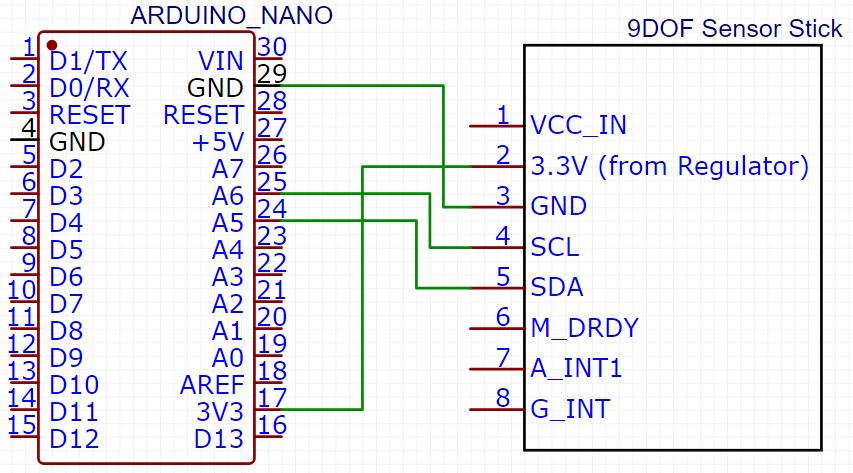
\includegraphics[height=0.3\textheight]{image/schema.png}
    \caption\centering{Schéma zapojení senzoru GY - 85}
\end{figure}

\subsection{9 DOF senzor - GY-85}
Tento model senzoru jsem si původně vybral pro využití gyroskopu, ale v průběhu projektu bylo jasné že nefunguje perfektně. Gyroskop na této desce totiž vypisuje stupňe za sekundu. Zpracování této hodnoty je složité a nepřesné, tudíž není gyroskop ideální pro tento typ ovladače. Místo toho jsem proto použil akcelerometr který je přítomen na stejné desce. Díky knihovny pro GY-85 bylo programování velice snadné. Naklonění ovladače se tak dalo jednoduše vypočítat přes vzorec za pomoci proměnných přečtených z akcelerometru:
\begin{lstlisting}[language={C++}, caption={C++ - Arduino kód pro vypočítání naklonění }, label={Script}]
rolldeg = 180 * (atan(Y / sqrt(X * X + Z * Z))) / PI;
\end{lstlisting}

\chapter{Spojení hardware a unity}
\section{Automatické detekování portu arduina}
Abychom v unity mohli příjmout data z arduina musíme nejprve otevřít serial port ,přes který poté budeme číst. C\# má díky knihovně System možnost přečíst všechny připojené "COM porty" pomocí "SerialPort.GetPortNames();". \\ 
Problém však je že to tyto available porty hodí do listu. Za předpokladu že uživatel používá pouze jeden ovladač jsem použil for loop který postupně zkouší všechny available porty dokud nenajde nějaký ze kterého lze číst. (arduino)

\begin{lstlisting}[language={[Sharp]C}, caption={C\# skript pro automatické nalezení komunikačního portu arduina}, label={Script}]
// list all serial ports
ports = SerialPort.GetPortNames();
    for (int i = 0; i < ports.Length; i++){
            portName = ports[i];
            data_stream = new SerialPort(portName, 9600);
            Debug.Log(portName);
            // open port that got found
            try
            {
                data_stream.Open();
                portFound = true;
                break;
            }
            catch (Exception e)
            {
                Debug.Log("Failed to open port " + portName + ": " + e.Message);
            }
        }

    if (!portFound)
    {
        Debug.LogError("Failed to find a valid COM port.");
    }
}
\end{lstlisting}

\subsection{Čtení dat z portu arduina a nastavení rychlosti hráče}
Následující kód převezme data z arduina a nastaví je jako force v unity, čímž pohne tělesem, v našem případě objektem hráče.
    \begin{lstlisting}[language={[Sharp]C}, caption={C\# skript pro přečtení a nastavení rychlosti pro hráče}, label={Script}]
    //read arduino data
        receivedString = data_stream.ReadLine();
        string[] datas = receivedString.Split(','); //split the data between ','
        rb.AddForce(0, 0, float.Parse(datas[1]) * sensitivity * Time.deltaTime, ForceMode.VelocityChange);
        rb.AddForce(float.Parse(datas[0]) * sensitivity * Time.deltaTime, 0, 0, ForceMode.VelocityChange);
\end{lstlisting}


	\chapter*{Závěr}
	
	Cílem projektu bylo vytvořit automaticky generovaný labyrint s automatickou generací cíle. Tento cíl jsem splnil, dokonce jsem během projektu přidal časti hry které mě z počátku nenapadly, jako například hardwarový ovladač a automatické generování překážek, které jsem také splnil. Práce mi také umožnila naučit se programovat v jazyce C\# a uplatnit tyto znalosti v praxi. Dále jsem se naučil pracovat s knihovnami pro arduino. \\
    V budoucnu bych rád přidal:
    \begin{itemize}
    \item Pohyblivé překážky - momentální překážky jsou příliš statické a proto jsou lehce překonatelné pro hráče. Proto bych rád přidal překážky které by následovali náhodně generovanou cestu, tím by se obtížnost hry určitě zvýšila.
    \item Více obtížností - v aktuální verzi hry jsou pouze dvě obtížnosti, konkrétně 10x10 a 20x20. V budoucnu bych chtěl přidát další obtížnosti, které by si hráč musel postupně odemnkout pokořením předešlých obtížností.
    \item Body v labyrintu - Hráč má momentálně jediný cíl a tím je se dostat do cíle. S přídáním bodů, nebo klíčů které by odemkly cíl potom co by je hráč posbíral by se stala hra trochu zábavnější a těžší.
    \end{itemize}

 \renewcommand{\bibname}{Seznam použitých zdrojů}
	%% zdroje
	\begin{thebibliography}{99}
		\bibitem{wikipedia} Depth-first search wikipedia. [online]. Aktualizováno 23.11. 2023. [cit. 2024-01-11]. Dostupné z: \url{https://en.wikipedia.org/wiki/Depth-first_search}. 
		\bibitem{CsharpReference} C\# reference. [online]. © Microsoft 2023. Dostupné z: \url{https://learn.microsoft.com/en-us/dotnet/csharp/language-reference/}. [cit. 2024-01-11].
		\bibitem{arduinoForum} Arduino forum. [Online]. © 2020 Arduino. Dostupné z: \url{https://forum.arduino.cc/}. [cit. 2024-01-11].
		\bibitem{arduinoStackExchange} Arduino stack exchange. [online]. © 2024 Stack Exchange Inc. Dostupné z: \url{https://arduino.stackexchange.com/}. [cit. 2024-01-11].
        \bibitem{copilotTvurceObrazku} Copilot tvůrce obrázků. [online]. © 2024 Microsoft. Dostupné z: \url{https://copilot.microsoft.com/images/create}. [cit. 2024-01-11].
	\end{thebibliography}
	
	%% obrázky 
	\listoffigures
	
	%% tabulky
	%%\listoftables
	
	%%\appendix %% začínají přílohy
	
	%%\titleformat{\chapter}[block]{\scshape\bfseries\LARGE}{Příloha \thechapter}{10pt}{\vspace{0pt}[\vspace{-22pt}] %% nastavení nadpisu u příloh
	
	
	%%\chapter{%Příloha A 
		%%Spot diagramy a další }
	
	
\end{document}